\section{Weekly Meeting Logistics}

You're the manager of an animal shelter, which is run by a few full-time staff members and a group of $n$ volunteers. Each of the volunteers is scheduled to work one shift during the week. There are different jobs associated with these shifts (such as caring for the animals, interacting with visitors to the shelter, handling administrative tasks, etc.), but each shift is a single contiguous interval of time. Shifts cannot span more than one week (e.g., we cannot have a shift from 10 PM Saturday to 6 AM Sunday). There can be multiple shifts going on at once.

You'd like to arrange a weekly meeting with your staff and volunteers, but you have too many volunteers to be able to find a meeting time that works for everyone. Instead, you'd like to identify a suitable subset of volunteers to instead attend the weekly meeting. You'd like for every volunteer to have a shift that overlaps (at least partially) with a volunteer who is attending the meeting. Your thinking is that you can't personally meet with every single volunteer, but you would like to at least meet with people who have been working with every volunteer (and may be able to let you know if a volunteer is disgruntled or having any difficulties with their performance, etc.). Because your volunteers are busy people, you want to accomplish this with the fewest possible volunteers.

Your volunteer shifts are given as an input list $V$, and each volunteer shift $v_i$ is defined by a start and finish time $(s_i, f_i)$. Your goal is to find  the smallest subset of volunteer shifts such that every shift in $V$ overlaps with at least one of the chosen shifts. A shift $v_i=(1,4)$ overlaps with the shift $v_j=(3,5)$ but not with the shift $v_k=(4,6)$. 

\begin{questions}
\question[2] Your co-worker proposes the following greedy algorithm to select volunteers for your meeting:
\begin{quote}
    Select the shift $v$ that overlaps with the most other shifts, discard all shifts that overlap with $v$, and recurse on the remaining shifts.
\end{quote}
Give and briefly explain a counterexample to prove that this greedy strategy is not optimal.

\ifsolutions\begin{soln}
	Consider the instance:

	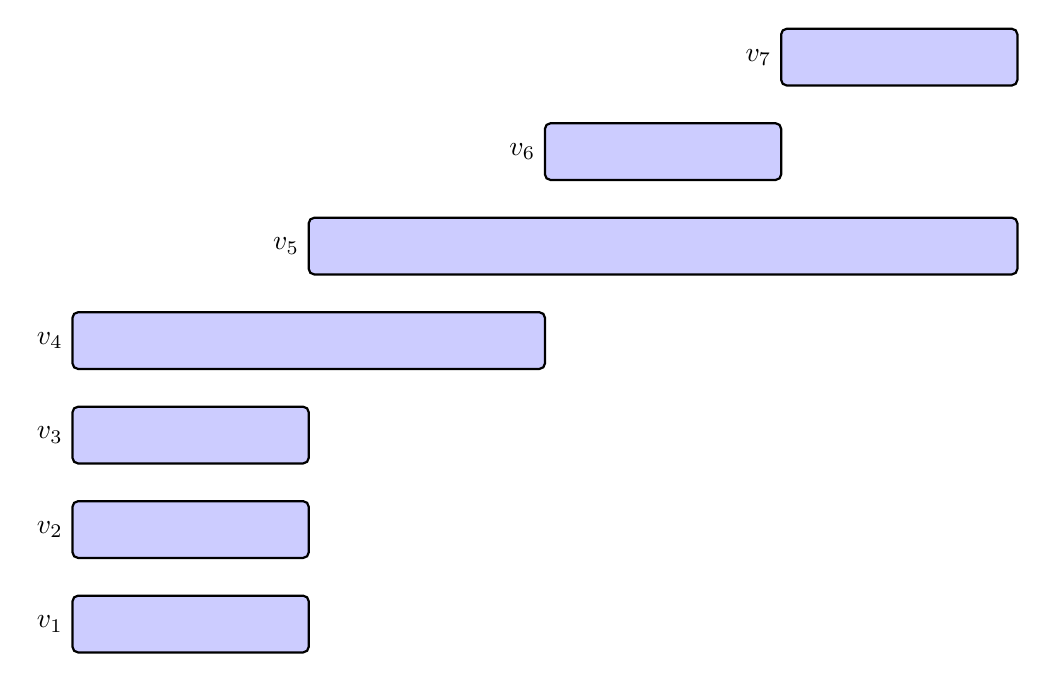
\begin{tikzpicture}[xscale=3, yscale=1.2]

		% Draw each interval as a bar
		\foreach \name/\start/\end/\y in {
				v_1/0/1/1,
				v_2/0/1/2,
				v_3/0/1/3,
				v_4/0/2/4,
				v_5/1/4/5,
				v_6/2/3/6,
				v_7/3/4/7
			} {
				\draw[thick, fill=blue!20, rounded corners=2pt] (\start,\y) rectangle (\end,\y+0.6);
				\node[left] at (\start,\y+0.3) {\(\name\)};
			}

	\end{tikzpicture}


	We see that in the proposed greedy algorithm that \(v_4\) intersects with the most amount of shifts, \(4\).

	After removing all intersections, only \(v_6, v_7\) remains, since those two are disjoint, the greedy algorithm returns volunteers \(v_4, v_6, v_7\) as its best solution.

	But notice that, by taking volunteers the two \(v_1, v_5\) we sufficiently cover all shifts in the set, thus this greedy algorithm is not optimal on all instances.

\end{soln}
\fi 

\question[3] Give a greedy algorithm to solve this problem. Give an unambiguous specification of your algorithm using  a \textbf{brief, plain English description}. Do not write pseudocode or worry about implementation details yet. (You may do this in part 5 if you feel that it's necessary to achieve a particular runtime.)

\ifsolutions\begin{soln}
	Sort the shifts in terms of ascending order by finish time, for any ties, place first the earliest start time.

	Choose the first shift in the ordered list, and add it to our solution set.

	Then delete any intersecting shifts to that shift and remove that shift itself from the ordered list.

	Continue to the next shift in the ordered list and repeat the previous steps until the list is empty.
\end{soln}

\fi 

\question[2] In this and the next question, you will prove the correctness of your greedy algorithm. To start, give a ``greedy stays ahead'' lemma that you can use to prove that your greedy algorithm is optimal. You do not need to prove the lemma (that comes next). Your lemma should compare a partial greedy solution to a partial optimal solution and describe some way in which the partial greedy solution is ``ahead.''

\ifsolutions\begin{soln}
	Denote the greedy solution by \(G = (g_1, g_2, \dots, g_k)\). Where we have chosen \(k\) shifts from the set \(V\).

	Lemma: At time \(f(g_i)\), greedy has less or as many volunteer shifts chosen than the optimal solution.
\end{soln}
\fi

\question[4] Prove the correctness of your algorithm. That is, prove that your set of selected shifts will (a) overlap with all the shifts in $V$, and (b) contains as few shifts as possible. You should do this by proving the greedy stays ahead lemma you stated in the previous question and using it to prove that the greedy solution is optimal.

\ifsolutions\begin{soln}
	We prove the lemma by induction on \( i \), where \( i \leq \min(k, l) \), and \( G = (g_1, g_2, \dots, g_k) \), \( O = (o_1, o_2, \dots, o_l) \) are the greedy and optimal solutions respectively, both sorted in increasing order of finish time.

	\textbf{Base Case (\(i = 1\)):}
	The greedy algorithm selects the shift with the earliest finish time among all shifts. Since \( o_1 \) is a valid first choice in some optimal solution, the greedy algorithm must finish no later:
	\[
		f(g_1) \leq f(o_1)
	\]

	\textbf{Inductive Hypothesis:}
	Assume for some \( i \geq 1 \), we have:
	\[
		f(g_j) \leq f(o_j) \quad \text{for all } j \leq i
	\]

	\textbf{Inductive Step (\(i + 1\)):}
	We want to show that \( f(g_{i+1}) \leq f(o_{i+1}) \).

	Let \( t \) be the earliest time after which both greedy and optimal resume selecting shifts — that is, the time immediately after \( f(g_i) \). Let \( S \) be the set of remaining unprocessed shifts that do not overlap with \( g_1, \dots, g_i \).

	By the inductive hypothesis, \( f(g_i) \leq f(o_i) \), so any shift in \( O \) that does not overlap with \( o_1, \dots, o_i \) must also not overlap with \( g_1, \dots, g_i \) — i.e., it is in \( S \). In particular, \( o_{i+1} \in S \).

	Now the greedy algorithm chooses \( g_{i+1} \) as the shift in \( S \) with the **earliest finish time**. Since \( o_{i+1} \in S \), we must have:
	\[
		f(g_{i+1}) \leq f(o_{i+1})
	\]

	Thus, the inductive step holds.

	\textbf{Conclusion:}
	By induction, we have shown that for all \( i \leq \min(k, l) \), it holds that:
	\[
		f(g_i) \leq f(o_i)
	\]

\end{soln}
\fi 

\question[4] Briefly justify a good asymptotic bound on the runtime of your algorithm. If you prefer to present pseudo-code to help track the runtime incurred, you may do so.

\ifsolutions\begin{soln}
	First, we sort the list \( V \) of \( n \) shifts in ascending order by their finish times. This takes \( O(n \log n) \) time.

	Then we iterate through the list from left to right and start selecting shifts, once a shift has been selected we add it to the solution set.
	The first shift is always selected.

	Next, we traverse to find the next selected shift in the ordered list that does not intersect with it.

	Intersection can be checked in \(O(1)\) time, by verifying that the selected shifts finish time is after the start time of the current potential candidate shift we are looking at.

	Notice in this process, each shift is visited at most once, either it is selected and added to the solution, or it is skipped due to intersection. Thus, the total traversal takes \( O(n) \) time.

	Combining both steps, the overall runtime of the algorithm is: \(O(n \log n + n) = O(n \log n)\).
\end{soln}













\fi 

\end{questions}